%Página
\section{Hierarquia de CAs}

O diagrama na Figura \ref{fig:ca} ilustra a hierarquia entre as CAs, incluindo a CA Root, a CA Intermediária e o Usuário Final. Cada um desses elementos possui características e funcionalidades específicas, que serão detalhadas a seguir.

\begin{figure}[H]
	\centering
	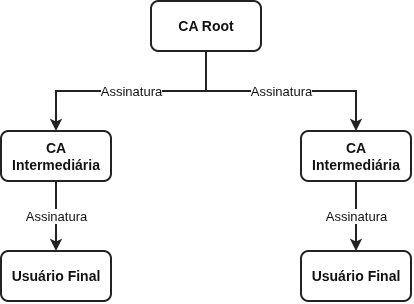
\includegraphics[scale=0.63]{ca.png}
	\caption{Hierarquia de CAs}
	\label{fig:ca}
\end{figure}

\subsection{Autoridade de Certificação (CA) Root}

Uma \textbf{Autoridade de Certificação (CA) Root} é a entidade central em uma infraestrutura de chave pública (PKI) que emite os primeiros certificados digitais, criando a base para a cadeia de confiança que valida identidades digitais na internet e em outros sistemas de comunicação segura. A CA Root emite e valida os certificados digitais, que são utilizados para autenticar a identidade de usuários, dispositivos ou servidores. Estes certificados garantem que a comunicação entre duas partes seja segura e confiável.\\

\subsection{Autoridade de Certificação (CA) Intermediária}

Uma \textbf{Autoridade de Certificação (CA) Intermediária} é uma entidade que emite certificados digitais em nome de uma Autoridade de Certificação Raiz (CA Raiz). Ela atua como um intermediário entre a CA Raiz, que é altamente confiável e segura, e os usuários finais ou servidores que recebem os certificados.\\

\subsection{Usuário Final}

Dentro de uma estrutura de Infraestrutura de Chave Pública (PKI) e Autoridade Certificadora (CA), o \textbf{Usuário Final} refere-se à entidade que utiliza certificados digitais para realizar atividades seguras, como autenticação, assinatura digital ou criptografia de dados. Esse usuário final pode ser uma pessoa, um dispositivo, um serviço ou uma aplicação.\\

\pagebreak
